\documentclass{tufte-handout}

\title{Continuous Probabilistic Programming I: Semantics}



\author[]{Steven Holtzen\\s.holtzen@northeastern.edu}

%\date{28 March 2010} % without \date command, current date is supplied

%\geometry{showframe} % display margins for debugging page layout
\setcounter{secnumdepth}{1}

\usepackage{graphicx} % allow embedded images
  \setkeys{Gin}{width=\linewidth,totalheight=\textheight,keepaspectratio}
  \graphicspath{{graphics/}} % set of paths to search for images
\usepackage{amsmath,amssymb,amsthm}  % extended mathematics
\usepackage{booktabs} % book-quality tables
\usepackage{units}    % non-stacked fractions and better unit spacing
\usepackage{multicol} % multiple column layout facilities
\usepackage{lipsum}   % filler text
\usepackage{fancyvrb} % extended verbatim environments
  \fvset{fontsize=\normalsize}% default font size for fancy-verbatim environments
\usepackage{listings}
\usepackage{tikz}
\usepackage{mathpartir}
\usepackage{subcaption}
\usepackage{mdframed}
\usepackage{epigraph}
\usepackage{enumitem}
\usepackage{stmaryrd}

\usetikzlibrary{shapes.geometric}


\usepackage[ruled,linesnumbered]{algorithm2e}
\SetKwComment{Comment}{/* }{ */}
\newcommand{\indep}{\perp \!\!\! \perp}

\tikzset{
  treenode/.style = {shape=rectangle, rounded corners,
                     draw, align=center,
                     },
  root/.style     = {treenode, font=\Large, bottom color=red!30},
  env/.style      = {treenode, font=\ttfamily\normalsize},
  dummy/.style    = {circle,draw}
}

% tikz
\usetikzlibrary{patterns,calc,backgrounds}


% TIKZ
\tikzstyle{nnf}=[
  >=stealth,font=\small,auto,scale=0.7,every node/.style={scale=0.7}
]
\tikzstyle{extnode}=[
  draw,circle,inner sep=2pt,fill=white
]

\tikzstyle{leafnode}=[
  draw,fill=gray!20,inner sep=3.5pt
]
\tikzstyle{constnode}=[
  draw,fill=white,inner sep=3.5pt
]
\tikzstyle{label}=[
  fill=white,inner sep=2.5pt
]

\tikzstyle{acarrow}=[
    decoration={markings,mark=at position 1 with {\arrow[scale=0.6]{>}}},
    postaction={decorate},
    shorten >=0.4pt,
    >=latex,
    line width=0.1
]

\tikzstyle{bnarrow}=[
    decoration={markings,mark=at position 1 with {\arrow[scale=1.5]{>}}},
    postaction={decorate},
    shorten >=0.7pt,
    >=latex,
    line width=0.3
]
\tikzstyle{bayesnet}=[
  >=latex, thick, auto
]
\tikzstyle{bnnode}=[
  draw,ellipse,minimum size=7mm,inner sep=1pt,font=\small
]
\tikzstyle{cpt}=[
  font=\footnotesize
]

\tikzstyle{graph}=[
  >=stealth,font=\small,auto,scale=1,every node/.style={scale=1}
]
\tikzstyle{node}=[
  draw,circle,inner sep=3pt,fill=white
]

% BDDs

\tikzstyle{bdd}=[
  >=latex, thick, >=stealth, font=\small,auto,scale=0.9,every node/.style={scale=0.9}
]
\tikzstyle{bddnode}=[
  draw,circle,inner sep=0pt,fill=white,minimum size=5.5mm
]

\tikzstyle{bddtriangle}=[
  draw, regular polygon, regular polygon sides = 3,inner sep=1pt,fill=white,minimum size=5.5mm
]

\tikzstyle{highedge}=[
    line width=0.9
]
\tikzstyle{lowedge}=[
    line width=0.9,dotted
]
\tikzstyle{bddterminal}=[
  draw,fill=gray!20,inner sep=2.5pt, font=\small
]

\lstdefinestyle{compact}{
  \ttfamily\tiny
}


\usetikzlibrary{positioning}

\newtheorem{theorem}{Theorem}
\newtheorem{definition}{Definition}
\newtheorem{conjecture}{Conjecture}
\newtheorem{lemma}{Lemma}
\newtheorem{exercise}{Exercise}
\newtheorem{remark}{Remark}


\usepackage{xcolor}

\definecolor{codegreen}{rgb}{0,0.6,0}
\definecolor{codegray}{rgb}{0.5,0.5,0.5}
\definecolor{codepurple}{rgb}{0.58,0,0.82}
\definecolor{backcolour}{rgb}{0.95,0.95,0.92}

\lstdefinestyle{mystyle}{
    backgroundcolor=\color{backcolour},   
    commentstyle=\color{codegreen},
    keywordstyle=\color{magenta},
    numberstyle=\tiny\color{codegray},
    stringstyle=\color{codepurple},
    basicstyle=\ttfamily\footnotesize,
    breakatwhitespace=false,         
    breaklines=true,                 
    captionpos=b,                    
    keepspaces=true,                 
    numbers=left,                    
    numbersep=5pt,                  
    showspaces=false,                
    showstringspaces=false,
    showtabs=false,                  
    tabsize=2
}

\lstset{style=mystyle}

\newcommand{\defn}[1]{\textbf{#1}}
\newcommand{\dbracket}[1]{\left \llbracket {#1} \right \rrbracket}
\newcommand{\dist}[1]{\mathtt{Dist}(#1)}
\newcommand{\true}[0]{\texttt{true}}
\newcommand{\te}[0]{\texttt{e}}
\newcommand{\false}[0]{\texttt{false}}
\newcommand{\real}[0]{\mathbb{R}}
\newcommand{\rational}[0]{\mathbb{Q}}
\newcommand{\lebesgue}[0]{\mathbb{L}}
\newcommand{\eval}[0]{\mathrm{ev}}
\newcommand{\disc}[0]{\textsc{Disc}}
\newcommand{\borel}[0]{\mathcal{B}}
\newcommand{\ent}[0]{\mathbb{S}}
\newcommand{\prog}[0]{\texttt{p}}
\newcommand{\bool}[0]{\mathbb{B}}
\newcommand{\cont}[0]{\textsc{Cont}}
\newcommand{\prop}[0]{\textsc{Prop}}
\newcommand{\bdd}[0]{\textsc{Bdd}}
\newcommand{\robdd}[0]{\textsc{Robdd}}
\newcommand{\compiles}[0]{\rightsquigarrow}

\newcommand{\bddtriangle}[1]{
    \begin{tikzpicture}
    \node [bddtriangle] {#1};
    \end{tikzpicture}}
\newcommand{\bddtrue}[0]{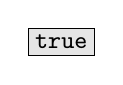
\begin{tikzpicture}
      \node [bddterminal] {$\true$};
    \end{tikzpicture}}
\newcommand{\bddfalse}[0]{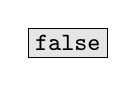
\begin{tikzpicture}
      \node [bddterminal] {$\false$};
    \end{tikzpicture}}


% Standardize command font styles and environments
\newcommand{\doccmd}[1]{\texttt{\textbackslash#1}}% command name -- adds backslash automatically
\newcommand{\docopt}[1]{\ensuremath{\langle}\textrm{\textit{#1}}\ensuremath{\rangle}}% optional command argument
\newcommand{\docarg}[1]{\textrm{\textit{#1}}}% (required) command argument
\newcommand{\docenv}[1]{\textsf{#1}}% environment name
\newcommand{\docpkg}[1]{\texttt{#1}}% package name
\newcommand{\doccls}[1]{\texttt{#1}}% document class name
\newcommand{\docclsopt}[1]{\texttt{#1}}% document class option name
\newenvironment{docspec}{\begin{quote}\noindent}{\end{quote}}% command specification environment



\begin{document}
\maketitle% this prints the handout title, author, and date


\begin{itemize}
  \item We give a syntax for a tiny continuous PPL called \textsc{TinyCont}:
\end{itemize}
\begin{lstlisting}[mathescape=true]

// expression terms
e ::=
  | $x$                // identifiers
  | $\real$               // real values
  | true | false
  | unif             // uniform distribution on the interval
  | return e
  | x $\leftarrow$ e; e
  | e + e | e $<$ e
\end{lstlisting}

\paragraph{Typing rules} Types $\tau$ have the following inductive description:
\begin{align*}
  \tau ::= \real \mid \bool
\end{align*}

Terms have the following typing judgments:

\begin{mathpar}
  \inferrule{\Gamma(x) = \tau}{\Gamma \vdash x : \tau}
  \and
  \inferrule{}{\Gamma \vdash \real : \real}
  \and
  \inferrule{}{\texttt{unif} : \dist{\real}}
  \and 
  \inferrule{\Gamma \vdash \te : \tau}{\Gamma \vdash \texttt{return e} : \dist{\tau}}
  \and 
  \inferrule{\Gamma \vdash \te_1 : \dist{\tau} \and \Gamma \cup [x \mapsto \tau] \vdash \te_2 : \tau'}
  {\Gamma \vdash \texttt{let x = e$_1$ in e$_2$} : \tau'}
\end{mathpar}

An example program: 

\begin{lstlisting}[caption={Simple program.}, mathescape=true]
x $\leftarrow$ unif;
return x + 1
\end{lstlisting}


% \begin{lstlisting}[caption={Program with conditioning.}]
% let x = sample unif [0, 1] in
% let y = observe 1/2 from unif [0, x] in
% x
% \end{lstlisting}

\section{Denotational semantics}
\begin{itemize}
  \item Denotation of types. Base types have two possible interpretations: measurable spaces (i.e. pairs $(\Omega, \Sigma)$ where $\Omega$ is a set and $\Sigma$ is a $\sigma$-algebra on 
  $\Omega$:) and pure 
  values. We denote the measurable space interpretation $\dbracket{\cdot}_M$:
  \begin{align*}
    \dbracket{\bool}_M &= (\{\true, \false\}, 2^{\{\true, \false\}}) \\
    \dbracket{\real}_M &= (\{\real, \borel(\real)\})
  \end{align*}
  where $\borel$ are the standard Borel-sets on $\real$. We say $v \in \dbracket{\tau}$ 
  if $v$ is an element of the $\sigma$-algebra of $\dbracket{\tau}$.

  \item Pure denotation of types is denoted $\dbracket{\tau}_p$ and is traditional:
  \begin{align*}
    \dbracket{\bool}_p &= \{\true, \false\} \\
    \dbracket{\real}_p &= \real.
  \end{align*}

\item Denotational of distribution-typed terms has the form:
\begin{align}
  \dbracket{\Gamma \vdash \te : \dist{\tau}} &: \dbracket{\tau}_M \rightarrow [0, 1]
\end{align}

\item Denotation of pure terms has the a standard base type

\item Inductive definition:\marginnote{
  Some notation:
  \begin{itemize}
    \item Dirac delta on value $v$: $\delta_v$
    \item Lebesgue measure on a set $A$: $\lebesgue(A)$
  \end{itemize}
}
\begin{align*}
  \dbracket{v} &= v \\
  \dbracket{\texttt{return}~v} &= \delta_v\\
  \dbracket{\texttt{unif}}(A) &= \lebesgue(A \cap [0, 1]) \\
  \dbracket{x \leftarrow \te_1; \te_2}(A) &= 
  \int \dbracket{\te_1}(v) \dbracket{\te_2[v/x]}(A)~\mathrm{d}v \\
  \dbracket{\te_1 + \te_2} &= \dbracket{\te_1} + \dbracket{\te_2} \\
  \dbracket{\te_1 < \te_2} &= \begin{cases}
    \true \quad& \text{if } \dbracket{\te_1} < \dbracket{\te_2} \\ 
    \false & \text{otherwise.}
  \end{cases}
\end{align*}

\end{itemize}

\section{Operational semantics}

\begin{itemize}
  \item Following \citet{culpepper2017contextual}. An \emph{entropy space} is a
  measurable space $(\mathbb{S}, \Sigma_{\mathbb{S}})$ with meaure $\mu_\ent :
  \Sigma_\ent \rightarrow [0,1]$ and functions:
  % \marginnote{It's worth briefly
  % reviewing some analysis. The usual notation for integrating a
  % function $f : \real \rightarrow \real$ over a set $A \subseteq \real$ is
  % $\int_A f(x) \mathrm{d}x$. Formally, 
  % }
  \begin{align}
    \pi_U : \ent \rightarrow [0,1] \\
    \pi_R, \pi_L: \ent \rightarrow \ent
  \end{align} 
  such that the following equations hold:
  \begin{enumerate}
    \item $\mu_\ent (\ent) = 1$, and so for any $r \in \real^+$ it is the case that:
    \begin{align} 
      \int k \mu_\ent(\mathrm{d}\sigma) = k.
      \label{eq:value}
    \end{align}
    \item For any measurable function $f : [0,1] \rightarrow \real^+$,
    \begin{align}
      \int f(\pi_U(\sigma))~\mu_\ent(\mathrm{d}\sigma) = \int_{[0,1]} f(x) \lebesgue(\mathrm{d}x)
      \label{eq:meas}
    \end{align}
    \item For any measurable $g : \ent \times \ent \rightarrow \real^+$:
    \begin{align}
      \int g(\pi_L(\sigma), \pi_R(\sigma))~\mu_\ent(\mathrm{d}\sigma) = \int\int g(\sigma_1, \sigma_2) \mu_\ent(\mathrm{d}\sigma_1) \mu_\ent(\mathrm{d}\sigma_2)
    \end{align}
  \end{enumerate}
  \item We give a Hilbert-cube style semantics in the style of
  \citet{wand2018contextual}. The relation has the form:
  \begin{align}
    \sigma \vdash \te \Downarrow v
  \end{align}
  \item Inductive description:\marginnote{
    Notation:
    \begin{itemize}
      \item $\pi_L(\sigma)$: left project of $\sigma$. Similarly $\pi_R$ is right.
      \item $\mathbb{S}$: the entropy space $[0,1]^\mathbb{N}$
    \end{itemize}
  }
  \begin{mathpar}
    \inferrule{}{\sigma \vdash v \Downarrow v}
    \and
    \inferrule{\pi_U(\sigma) = r}{\sigma \vdash \texttt{unif} \Downarrow r}
    \and
    \inferrule{}{\texttt{return}~v} \Downarrow v 
    \and 
    \inferrule{\pi_L(\sigma) \vdash \te_1 \Downarrow v_1 \and 
    \pi_R(\sigma) \vdash \te_2[v_1/x] \Downarrow v_2}{\sigma \vdash x \leftarrow \te_2; \te_2 \Downarrow v_2}
  \end{mathpar}
  \item For a term of $\te$ of type $\dist{\tau}$,
  This defines an \emph{evaluation function} $\eval : \Sigma \rightarrow \te \rightarrow \dbracket{\tau}_p$ 
  that maps each (well-typed) term to the value that it steps to.
\end{itemize}

\begin{theorem}[Adequacy] If $\Gamma \vdash \te : \dist{\tau}$, then for any 
  $A \in \dbracket{\tau}_M$ it is the case that:
  $\int [\eval(\sigma, \te) \in A] ~\mu_\ent(\mathrm{d}\sigma) = \dbracket{\te}(A)$.
\end{theorem}
\begin{proof}
  Structural induction on monadic terms. Base cases:
  \begin{itemize}
    \item \texttt{return v}. Case analysis: 
    \begin{itemize}
      \item Assume $v \in A$. Then:
          \begin{align*}
           \int [\eval(\sigma, \texttt{return v}) \in A] ~\mu_\ent(\mathrm{d}\sigma) &= \int 1 ~\mathrm{d}\sigma  \\
           &= 1 & \text {By (\ref{eq:value})}\\
           &= \dbracket{\texttt{return v}}(A).
        \end{align*}
        Similar for the case $v \notin A$.
    \end{itemize}
    \item \texttt{unif}. Then:
    \begin{align*}
      \int [\eval(\sigma, \texttt{unif}) \in A] ~\mu_\ent(\mathrm{d}\sigma) &=
      \int [\pi_U(\sigma) \in A] ~\mu_\ent(\mathrm{d}\sigma) \\
      &= \int_{[0,1]} [x \in A]~\lebesgue(\mathrm{d}x) & \text{By (\ref{eq:meas})} \\ 
      &= \dbracket{\texttt{unif}}(A).
    \end{align*}
  \end{itemize}
\end{proof}

\bibliographystyle{plainnat}
\bibliography{../bib}


\end{document}